\documentclass[twoside,twocolumn]{article}
\usepackage[hmarginratio=1:1,top=32mm,columnsep=20pt]{geometry}
\usepackage[hang, small,labelfont=bf,up,textfont=it,up]{caption} 
\usepackage{amsmath}
\usepackage{booktabs}
\usepackage{enumitem}
\setlist[itemize]{noitemsep}
\usepackage{abstract}
\renewcommand{\abstractnamefont}{\normalfont\bfseries}
\renewcommand{\abstracttextfont}{\normalfont\small\itshape}
\usepackage{titlesec}
\renewcommand\thesection{\Roman{section}}
\renewcommand\thesubsection{\Alph{subsection}}
\renewcommand\thesubsubsection{\arabic{subsubsection}}
\titleformat{\section}[block]{\normalsize\bfseries\scshape\centering}{\thesection.}{1em}{}
\titleformat{\subsection}[block]{\normalsize\bfseries\centering}{\thesubsection.}{1em}{}
\titleformat{\subsubsection}[block]{\normalsize\centering}{\thesubsubsection.}{1em}{}
\usepackage{fancyhdr}
\pagestyle{fancy}
\fancyhead{}
\fancyhead[C]{Computational Physics Homework $\bullet$ May 2018 $\bullet$ Vol. I, No. 1}
\usepackage{titling}
\usepackage{hyperref}
\hypersetup{unicode}
\AtBeginShipoutFirst{\input{zhwinfonts.tex}}
\usepackage{bm}
\usepackage{braket}
\usepackage{CJKutf8}
\usepackage{xcolor}
\usepackage{dcolumn}
\usepackage{graphicx}
\usepackage{indentfirst}
\usepackage{listings}
\usepackage[toc, page, title, titletoc, header]{appendix}
\definecolor{grey}{rgb}{0.8,0.8,0.8}
\definecolor{darkgreen}{rgb}{0,0.3,0}
\definecolor{darkblue}{rgb}{0,0,0.3}
\def\lstbasicfont{\fontfamily{pcr}\selectfont\footnotesize}
\lstset{
	numbers=left,
	numberstyle=\small,
	escapeinside=``,
	showstringspaces=false,
	showspaces=false,
	tabsize=4,
	frame=single,
	basicstyle={\footnotesize\lstbasicfont},
	keywordstyle=\color{darkblue}\bfseries,
	identifierstyle=,
	commentstyle=\color{darkgreen},
	stringstyle=\color{black}
}
\lstloadlanguages{C,C++,Fortran,Java,Matlab,Mathematica,Python}
\setlength{\parindent}{2em}
\begin{document}
\begin{CJK*}{UTF8}{gkai}
%----------------------------------------------------------------------------------------
%	TITLE SECTION
%----------------------------------------------------------------------------------------

\setlength{\droptitle}{-4\baselineskip} % Move the title up
\pretitle{\begin{center}\Huge\bfseries} % Article title formatting
	\posttitle{\end{center}} % Article title closing formatting
\title{计算物理第一次作业} % Article title
\author{
	\textsc{梁旭民}\thanks{\noindent 指导老师:齐新老师} \\[1ex] % Your name
	\normalsize Cuiying Hornors College, Lanzhou University \\ % Your institution
	\normalsize \href{mailto:liangxm15@lzu.edu.cn}{liangxm15@lzu.edu.cn} % Your email address
}
\date{}
\renewcommand{\maketitlehookd}{
	\begin{abstract}
		本次计算物理作业有两个问题:第一个问题是求解数值积分,让我们学会处理被积函数在上下限取值处发散的问题,并简单体会不同数值积分方法精确度的优劣;第二个问题是运用二分法、Newton法、弦切法求解一个有无穷个解的超越方程并比较不同数值求解方程根的方法的收敛性快慢
	\end{abstract}
}
\maketitle

%----------------------------------------------------------------------------------------
%	SECTION 1
%----------------------------------------------------------------------------------------

\section{计算定积分}
\subsection{问题描述}
利用学到的积分方法计算以下积分,并讨论各种方案的计算精度。根据自己的程序,选择符合自己要求的积分方法。
\begin{equation*}
	\int_{0}^{1}t^{-\frac{2}{3}}(1-t)^{-\frac{1}{3}}dt=\frac{2\pi}{\sqrt{3}}
\end{equation*}
\subsection{问题分析}
观察被积函数我们发现:当$t=0$或$t=1$时,该被积函数会发散,因此我们首先将积分分段
\begin{equation*}
	\begin{aligned}
		\int_{0}^{1}t^{-\frac{2}{3}}(1-t)^{-\frac{1}{3}}dt=&\int_{0}^{\frac{1}{2}}t^{-\frac{2}{3}}(1-t)^{-\frac{1}{3}}dt\\&+\int_{\frac{1}{2}}^{1}t^{-\frac{2}{3}}(1-t)^{-\frac{1}{3}}dt
	\end{aligned}
\end{equation*}
为了避免积分在奇点处发散,我们分别做变量替换:
\subsubsection{第一部分积分}
令$x=t^{\frac{1}{3}}$,有$t=x^{3}$及$dt=3x^{2}dx$,则第一部分积分变为
\begin{equation*}
	\begin{aligned}
		&\int_{0}^{\frac{1}{2}}t^{-\frac{2}{3}}(1-t)^{\frac{1}{3}}dt\\
		&=\int_{0}^{(\frac{1}{2})^{\frac{1}{3}}}x^{-2}(1-x^{3})^{-\frac{1}{3}}3x^{2}dx\\
		&=\int_{0}^{(\frac{1}{2})^{\frac{1}{3}}}3(1-x^{3})^{-\frac{1}{3}}dx
	\end{aligned}
\end{equation*}
\subsubsection{第二部分积分}
令$x=(1-t)^{\frac{2}{3}}$,则第二部分积分变为
\begin{equation*}
	\begin{aligned}
		&\qquad \int_{\frac{1}{2}}^{1}t^{-\frac{2}{3}}(1-t)^{-\frac{1}{3}}dt\\
		&=-\int_{\frac{1}{2}}^{1}t^{-\frac{2}{3}}(1-t)^{-\frac{1}{3}}d(1-t)\\
		&=-\int_{0}^{\left(\frac{1}{2}\right)^{\frac{2}{3}}}(1-x^{\frac{3}{2}})^{-\frac{2}{3}}x^{-\frac{1}{2}}(-\frac{3}{2})x^{\frac{1}{2}}dx\\
		&=\int_{0}^{\left(\frac{1}{2}\right)^{\frac{2}{3}}}\frac{3}{2}(1-x^{\frac{3}{2}})^{-\frac{2}{3}}dx
	\end{aligned}
\end{equation*}
因此整个积分变成
\begin{equation*}
	\begin{aligned}
		&\int_{0}^{1}t^{-\frac{2}{3}}(1-t)^{-\frac{1}{3}}dt=\int_{0}^{(\frac{1}{2})^{\frac{1}{3}}}3(1-x^{3})^{-\frac{1}{3}}dx\\
		&\qquad +\int_{0}^{\left(\frac{1}{2}\right)^{\frac{2}{3}}}\frac{3}{2}\left(1-x^{\frac{3}{2}}\right)^{-\frac{2}{3}}dx
	\end{aligned}
\end{equation*}
接下来,我们分别用矩形法、梯形法和Simpson法进行计算,并对相同步长下的计算精度及计算速度进行简单分析。
\subsection{数据分析}
在不同的步长下得到矩形法、梯形法、Simpson法得到积分结果与标准值$\frac{2\pi}{\sqrt{3}}$之间的差距见Table 1.
\begin{table}[htbp]
	\centering
	\caption{不同步长下不同方法数值积分结果对比}
	\resizebox{\linewidth}{!}{
		\begin{tabular}{c|c|c|c|c|c|c}
			\hline
			步长 & \multicolumn{2}{c|}{Rectangle} & \multicolumn{2}{c|}{Trapezoid} & \multicolumn{2}{c}{Simpson} \\
			\hline
			N & I     & $I-I_{0}$ & I     & $I-I_{0}$ & I     & \multicolumn{1}{c}{$I-I_{0}$} \\
			\hline
			100 & 3.621660 & -0.005832 & 3.627536 & 0.000037 & 3.627599 & 0.000001 \\
			1000 & 3.627012 & -0.000587 & 3.627599 & 0.000000 & 3.627599 & 0.000000 \\
			10000 & 3.627540 & -0.000059 & 3.627599 & 0.000000 & 3.627599 & 0.000000 \\
			100000 & 3.627593 & -0.000006 & 3.627599 & 0.000000 & 3.627599 & 0.000000 \\
			1000000 & 3.627598 & -0.000001 & 3.627599 & 0.000000 & 3.627599 & 0.000000 \\
			\hline
		\end{tabular}}
		\label{tab:addlabel}
	\end{table}
	可以发现在步长相同的情况下,Simpson方法计算的结果精度远大于矩形法和梯形法,这可能是用抛物线拟合曲线时符合较好。同时可以得到结论梯形法的精度比矩形法高。
	
%----------------------------------------------------------------------------------------
	%	SECTION 2
%----------------------------------------------------------------------------------------
	
	\section{求解方程}
	\subsection{问题描述}
	求解非线性方程的根:
	\begin{equation*}
		E_{i}-V(r)=0
	\end{equation*}
	其中,$E_{i}=-0.40705$\\
	V的表达式为
	\begin{equation*}
		V_{et}(x)=-\frac{1}{x}e^{-\mu x}\cos(\mu x)\quad \mu=0.1
	\end{equation*}
	\subsection{问题分析}
	用Python绘制函数图像$y(x)=-0.40705+\frac{1}{x}e^{0.1 x}\cos(0.1 x)$,见Figure 1.
	\begin{figure}[h]
		\centering
		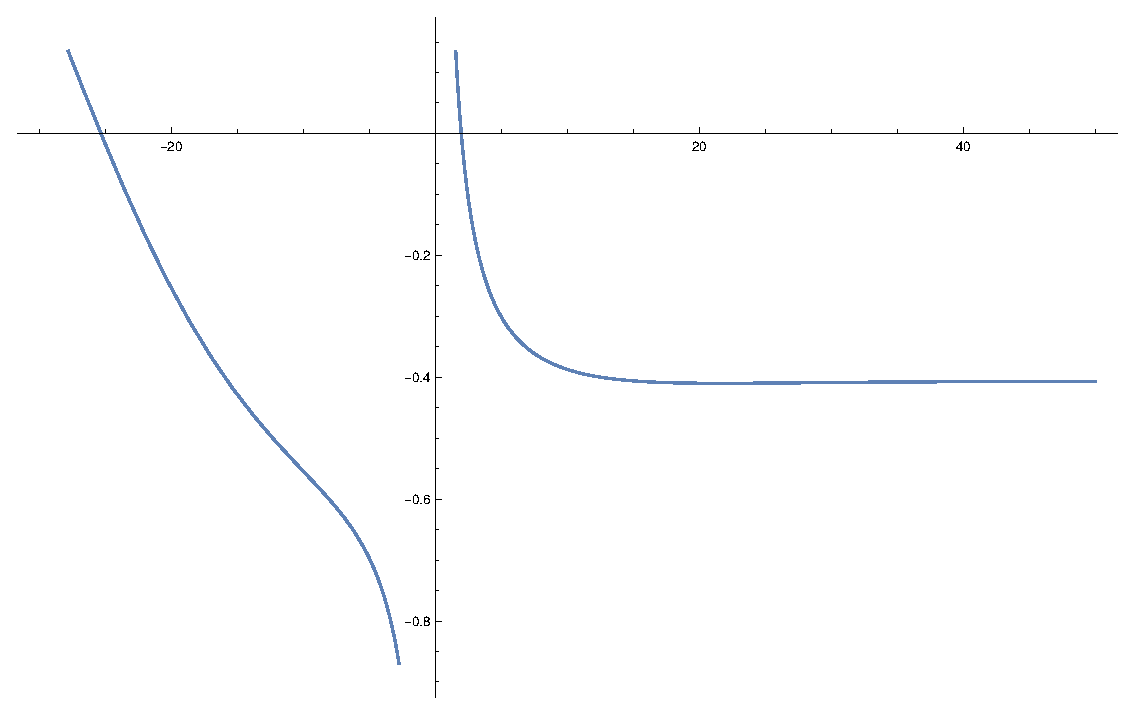
\includegraphics[width=0.8\linewidth]{./figure/figure}
		\caption{区间$[-30,50]$中的函数$f(x)$图像}
		\label{fig:figure_2}
	\end{figure}
	
	该函数零点有无穷多个,其中一个在$x=2$附近,因此我在分别用二分法,Newton法或弦切法讨论解的收敛性时,为了运算时间的缩小,选定x的取值区间[1.5,2.0],为了比较方便我用Mathematica求解出方程的其中一个根$x_{0}=1.9767881587790763$并作为标准值。
	\subsection{数据分析}
	我们选取$1\times 10^{-11}$作为可容忍误差,分别用二分法、Newton法和弦切法求解方程的[1.5,2.0]区间内的根及收敛补数与标准值的绝对误差见Table 2.
	\begin{table}[htbp]
		\centering
		\caption{方程数值解}
		\resizebox{\linewidth}{!}{
			\begin{tabular}{c|c|c|c}
				\hline&&&\\
				方法   & 二分法 & Newton法   & 弦切法    \\
				\hline&&&\\
				方程数值解 &1.9767881587758893 &1.9767881587790763 &1.9767881587790763  \\
				绝对误差$(\times 10^{-12})$  &$5.889289056426605$&$9.0762952709155797$&$9.0762952709155797$ \\
				收敛步数  &28 &5 &5 \\
			\end{tabular}}
			\label{tab:addlabel}
		\end{table}
		可以看出Newton法寻找方程解得收敛速度和弦切法差不多,而二分法要比这两种算法慢,同时由于Newton法需要求解函数的导数,因此相比而言弦切法这种算法较优。

%----------------------------------------------------------------------------------------
%	APPENDICES SECTION
%----------------------------------------------------------------------------------------

\newpage
\onecolumn
\begin{appendices}
\section{求解上下限发散的数值积分}
这是运用矩形法、梯形法、Simpson法求解上下限发散的数值积分Python代码。\\
\textbf{\textcolor[rgb]{0.98,0.00,0.00}{Input Python source:}}
\lstinputlisting[language=Python]{./program/Integration.py}
\newpage
\section{求解非线性方程}
这是运用二分法、Newton法和弦切法求解非线性方程Python代码。\\
\textbf{\textcolor[rgb]{0.98,0.00,0.00}{Input Python source:}}
\lstinputlisting[language=Python]{./program/seq.py}
\end{appendices}

%----------------------------------------------------------------------------------------
%	REFERENCE
%----------------------------------------------------------------------------------------

\newpage
\renewcommand\refname{参考文献}
\begin{thebibliography}{99}
\bibitem{ref1}Philip J. Davis and Philip Rabinowitz, Methods of Numerical Integration.
\bibitem{ref2}George E. Forsythe, Michael A. Malcolm, and Cleve B. Moler, Computer Methods for Mathematical Computations. Englewood Cliffs, NJ: Prentice-Hall, 1977. (See Chapter 5.)
\bibitem{ref3}Press, W.H.; Teukolsky, S.A.; Vetterling, W.T.; Flannery, B.P. (2007), "Chapter 4. Integration of Functions", Numerical Recipes: The Art of Scientific Computing (3rd ed.), New York: Cambridge University Press, ISBN 978-0-521-88068-8.
\bibitem{ref4}Josef Stoer and Roland Bulirsch, Introduction to Numerical Analysis. New York: Springer-Verlag, 1980. (See Chapter 3.)
\bibitem{ref5}Boyer, C. B., A History of Mathematics, 2nd ed. rev. by Uta C. Merzbach, New York: Wiley, 1989 ISBN 0-471-09763-2 (1991 pbk ed. ISBN 0-471-54397-7).
\bibitem{ref6}Eves, Howard, An Introduction to the History of Mathematics, Saunders, 1990, ISBN 0-03-029558-0.
\bibitem{ref7} Wallis, John (1685). A Treatise of Algebra, both Historical and Practical. Shewing the Original, Progress, and Advancement thereof, from time to time, and by what Steps it hath attained to the Heighth at which it now is. Oxford: Richard Davis. doi:10.3931/e-rara-8842.
\bibitem{ref8}Raphson, Joseph (1697). Analysis Æequationum Universalis seu ad Æequationes Algebraicas Resolvendas Methodus Generalis, \& Expedita, Ex nova Infinitarum Serierum Methodo, Deducta ac Demonstrata (in Latin) (secunda ed.). London. doi:10.3931/e-rara-13516.
\bibitem{ref9}Ryaben'kii, Victor S.; Tsynkov, Semyon V. (2006), A Theoretical Introduction to Numerical Analysis, CRC Press, p. 243, ISBN 9781584886075.
\bibitem{ref10}Kaw, Autar; Kalu, Egwu (2008), Numerical Methods with Applications (1st ed.).
\bibitem{ref11}Allen, Myron B.; Isaacson, Eli L. (1998). Numerical analysis for applied science. John Wiley \& Sons. pp. 188–195. ISBN 978-0-471-55266-6.
\end{thebibliography} 

%----------------------------------------------------------------------------------------
\end{CJK*}
\end{document}
